
El algoritmo mostrado en la secci\'on anterior fue implementado en \emph{Python 3.6.3} aprovechando de la versatilidad que este proporciona, principalmente, porque a las variables no es necesario especificar un tipo ya que este se asigna al momento de crearla dependiendo del elemento a almacenar, algo que en otros lenguajes como Java se solucionar\'ia con sobrecarga de m\'etodos y varias variables con los tipos a utilizar, tomando en consideraci\'on esto, solo se defini\'o una clase \emph{nodo}, donde una variable miembro es la que almacena la informaci\'on del nodo independientemente del contenido de \'este, tambi\'en, se almacena el tiempo de retraso de espera para realizar la acci\'on y un contador del n\'umero de veces que se ha usado ese nodo. Y como se mencion\'o, se utiliza un grafo dirigido y en ning\'un momento es necesario leer el grafo en sentido contrario, por lo que dentro de la clase solo se almacena una lista de nodos a los que apunta. 


Para realizar la b\'usqueda de un nodo en espec\'ifico en el grafo, se utiliza un diccionario con los nodos existentes en \'el, de este modo no importa el tama\~no o lo revuelto que este el grafo, no es necesario realizar un recorrido para localizar un nodo en espec\'ifico.


El software fue dividido en 4 partes; \emph{monitoreo}, \emph{respaldo}, \emph{carga} y \emph{ejecuci\'on}. En el \emph{monitoreo} se hace uso de la biblioteca \emph{pyinput} en su versi\'on 1.3.9 la cual por medio de 2 hilos; uno para el monitor del teclado y otro para el monitor del rat\'on, se capturan las acciones que el usuario realice en la computadora con estos dos dispositivos. En el primero se capturan las acciones de presionar (pressed) o liberar (released) una tecla, mientras que para el segundo se tienen m\'as tipos de acciones (presionar, liberar, mover (move) y rueda (scroll)), entre las cuales, mover, captura coordenadas bidimensionales y la rueda, se mueve arriba o abajo. 


Al detectar alguna de las acciones mencionadas se registra la informaci\'on correspondiente (Tiempo de espera, acci\'on, [tecla, bot\'on, coordenadas o direcci\'on del scroll]) en una lista en memoria, posteriormente un hilo de procesamiento lee la lista e intenta crear el nodo o en caso de que el nodo ya exista se debe buscar dicho nodo en el grafo y verificar que la relaci\'on con el nodo anterior. Adem\'as, se evalua si la secuencia es candidata para formar parte de una secuencia, en caso dado se almacenara en una lista temporal y posteriormente si la secuencia es una tarea repetitiva, se almacenara en otra lista para poder contabilizar las repeticiones de esta y mostr\'arsela al usuario, si est\'e decide que si es una tarea \'util, esta se almacenara en otro diccionario con el comando que decida el usuario como llave, en caso contrario se mete a una lista de secuencias ignoradas para evitar mostrarlas de nuevo.


El \emph{respaldo} lee la lista de acciones, el diccionario de tareas y la lista de secuencias ignoradas anteriormente mencionadas y las almacena en archivos de texto, para realizar esta tarea fue necesario asignarla a un hilo de ejecuci\'on que realizara la tarea cada 120 segundos. La \emph{carga} se ejecuta una sola vez al iniciar el programa leyendo los archivos mencionados (en caso de existir), empezando con la lista de acciones realizadas por el usuario, para reconstruir el grafo, pero sin realizar la b\'usqueda de tareas, posteriormente, las tareas guardadas se vuelven a colocar en el diccionario de tareas y finalmente se rellena la lista de las secuencias ignoradas, restaurando el sistema tal cual estaba antes de finalizar el programa.


Para la \emph{ejecuci\'on} se desarroll\'o una interfaz gr\'afica simple con \emph{TkInter} para que el usuario interact\'ue con el software, en la figura \ref{fig:v01} se observa la ventana principal y desde la parte superior se aprecia al asistente amarillo creado para esta aplicaci\'on sobre una lista con algunas tareas identificables por n\'umeros y en la parte inferior un bot\'on para que la computadora realice la tarea seleccionada en la lista, para lo cual se defini\'o un diccionario con los comandos posibles para que se traduzcan del texto capturado al comando ejecutable. 


\begin{figure}[H]
\centering
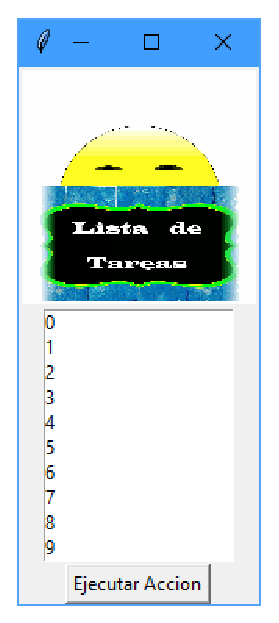
\includegraphics[width=0.2\columnwidth]{chap4/Imagenes/ventana1.eps}
\caption{Ventana principal con el asistente y una lista de tareas guardadas.}
\label{fig:v01}
\end{figure} 

Al momento de detectarse una tarea repetitiva, se le muestra al usuario una ventana de captura muy similar a la de la figura \ref{fig:v02}, en la cual se aprecia al mismo asistente amarillo con otro letrero y la secuencia obtenida, tambi\'en se observa un cuadro de texto para introducir el nombre solicitado, mas abajo se localizan los botones para guardar la tarea y agregarla a la lista de la figura \ref{fig:v01} o ignorarla.


\begin{figure}[H]
\centering
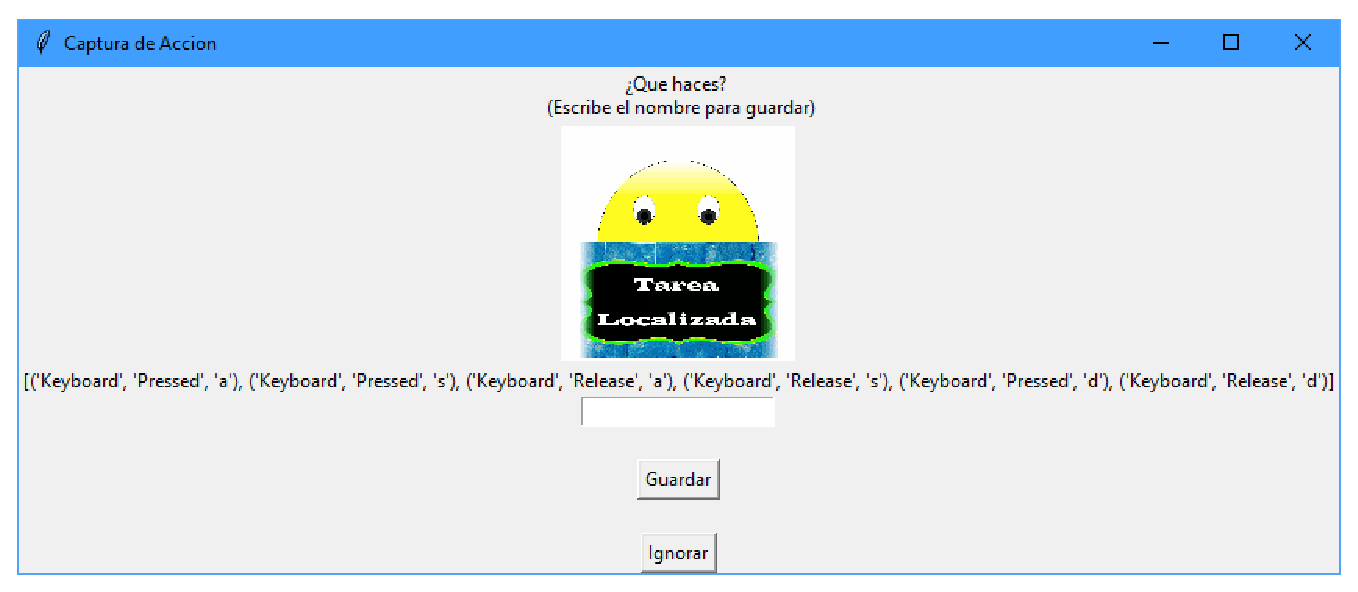
\includegraphics[width=0.9\columnwidth]{chap4/Imagenes/ventana2.eps}
\caption{Ventana mostrando una tarea encontrada.}
\label{fig:v02}
\end{figure}

A continuaci\'on se presenta el pseudo--codigo del programa desarrollado.

\begin{table}[]
\begin{lstlisting}
Procedimiento monitoreo
Mientras Verdad Hacer
    Nodo = Capturar accion de teclado o raton
    Si Nodo existe en grafo Entonces
        Incrementar contador_Nodo
    Si no Entonces
		Colocar Nodo en grafo
		Si contador_nodo > 70 Entonces
			Si Nodo existe en Secuencia Entonces
				Si Secuencia existe en Lista_secuencias Entonces
					Si contador_Secuencia > 5 Entonces
						Escribir ``Si desea Guardar la tarea [Secuencia], escriba un nombre''
						Leer Respuesta
						Si Respuesta es nombre Entonces
							Agregar Secuencia a Lista_Tareas
						Si no Entonces 
							Agregar Secuencia a Lista_Ignoradas
					Si no Entonces
					Incrementar contador_Secuencia
				Si no Entonces
					Agregar Secuencia a Lista_Secuencias
            Borrar Secuencia
            Si no Entonces
		        Agregar nodo a Secuencia
		Si no Entonces
            Borrar Secuencia
Fin Mientras
Fin Procedimiento 

Procedimiento Ejecucion
Mientras Verdad Hacer
Escribir ``Selecciona la tarea a ejecutar''
Leer Selecci\'on
Escribir ``Ejecutar Accion seleccionada?''
Leer Decisi\'on
Si Decisi\'on = ``Si'' Entonces
	Ejecutar Seleccion
Fin Mientras
Fin Procedimiento

\end{lstlisting}
\end{table}